\chapter{Pseudo-turbulence}\label{appendixa}

In chapter \ref{theory}, a phenomenon called pseudo-turbulence is discussed. 

In this work, simulations are done using OpenFOAM with the Euler-Euler model discussed in section \ref{eemodel}. The interphase momentum transfer model comes from \ref{eq:wenyudrag}, other forces were neglected.

The geometry was the same as the one from the work of Alexiadis et al. \cite{Alexiadis2012}, as shown in figure \ref{appendixgeometry1}.

\begin{figure}[H]
    \centering
    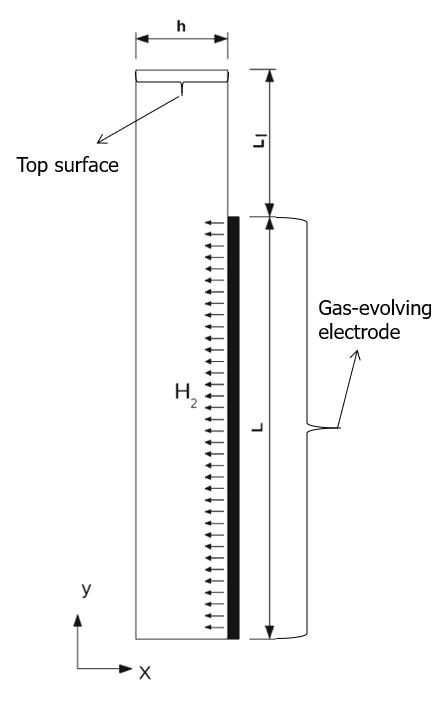
\includegraphics[scale = 0.7]{appendixgeometry1.png}
    \caption{Geometry of a quiescent channel, the sketch comes from Alexiadis et al. \cite{Alexiadis2012}, The bottom of the channel is set as wall and the top is a free surface, gas is evolved from the gas-evolving electrode at the right hand side of the channel, $L = 30 \, \mathrm{mm}$, $L1 = 20 \, \mathrm{mm}$, $h = 3 \, \mathrm{mm}$}
    \label{appendixgeometry1}
\end{figure}

\section*{Boundary conditions}


\paragraph{The gas-evolving electrode}
\*

At the gas-evolving electrode, the boundary condition can be given as:

\begin{equation}
    \alpha_d u_{dx} = - \frac{RTi_{av}}{2pF}, \quad i_{av} = 1000 \, \mathrm{A/m^2}
\end{equation}

\begin{equation}
    u_{dy} = 0 \, \mathrm{m/s}
\end{equation}

\begin{equation}
    \mathbf{u_{c}} = 0 \, \mathrm{m/s}
\end{equation}

As discussed in section \ref{modellingreview}, the gas volume fraction $\alpha_d$ remains unknown at the wall, here we simply assume $\alpha_d = 0.5$ as Alexiadis did. For pressure and volume fraction, $ \mathrm{zeroGradient}$ boundary condition is used in OpenFOAM.

\paragraph{The free surface}
\*

At the free surface, $ \mathrm{zeroGradient}$ is chosen as the boundary condition for the gas phase velocity in the y-direction, while for the liquid phase, it is slip boundary condition, which means the normal velocity is fixed to zero and the tangential velocity is $ \mathrm{zeroGradient}$. For pressure and volume fraction, $ \mathrm{zeroGradient}$ boundary condition is also used.

\section*{Results}

\begin{figure}[H]
    \centering
    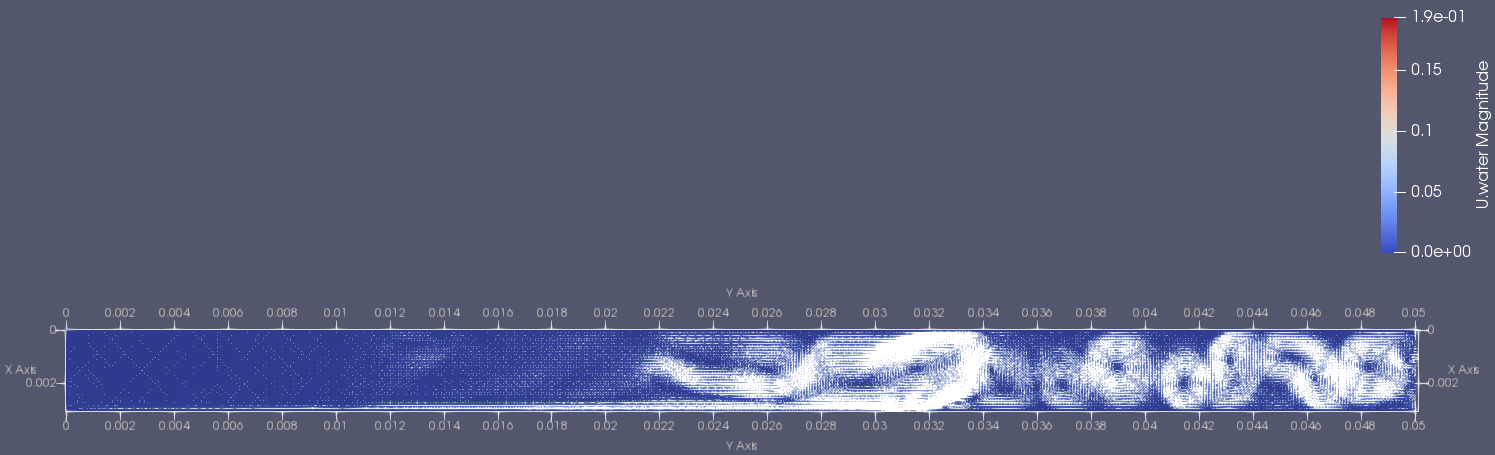
\includegraphics[width=\textwidth]{velocitycontourpseudoturbulence.png}
    \caption{The velocity contour in the quiescent channel, the contour is rotated 90 degree clockwise}
    \label{contourpt}
\end{figure}

\begin{figure}[H]
    \centering
    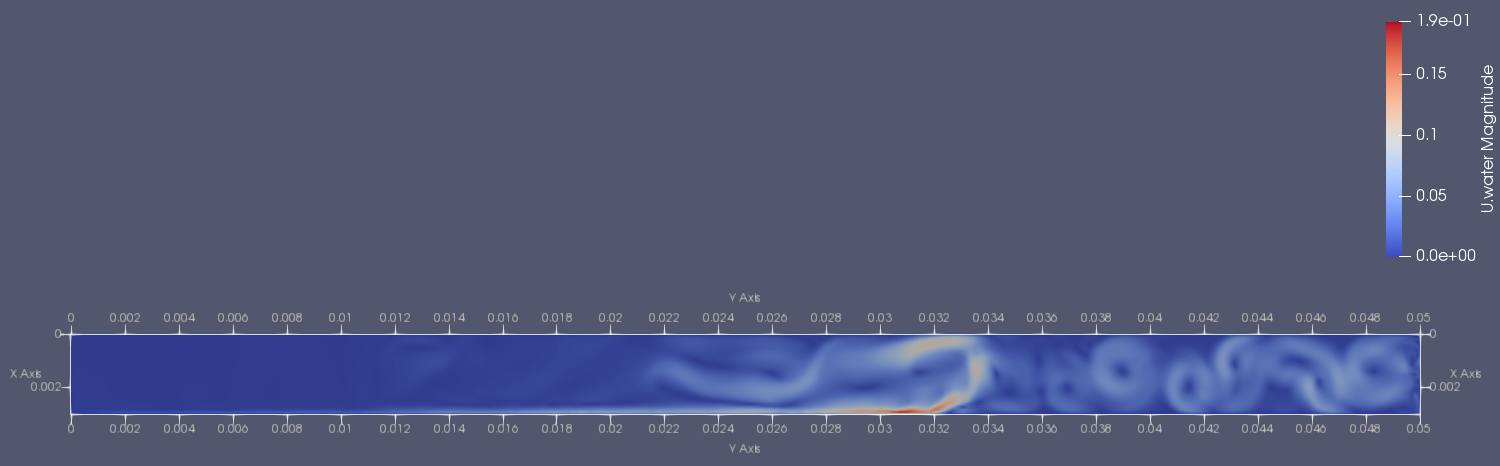
\includegraphics[width=\textwidth]{velocitywithoutarrow.png}
    \caption{The velocity magnitude contour in the quiescent channel without arrows, the contour is rotated 90 degree clockwise}
    \label{contourptnoarrow}
\end{figure}


From figure \ref{contourpt} and \ref{contourptnoarrow} we can see the similar phenomena as shown in figure \ref{pseudo}. However, in the simulation results from Alexiadius, the vortices filled the whole channel, as shown in figure \ref{pseudoalex}, while in this work, vortices only fill the top half of the channel. 

The reason for this discrepancy is still unclear, but an assumed claim from the simulation results in this thesis work could be that the triggering of pseudo-turbulence might have a direct relation to the local volume fraction value \cite{Boissonneau2000}. In other words, the volume fraction might need to be included in the criterion in equation \ref{ptcriterion} as well.

\begin{figure}[H]
    \centering
    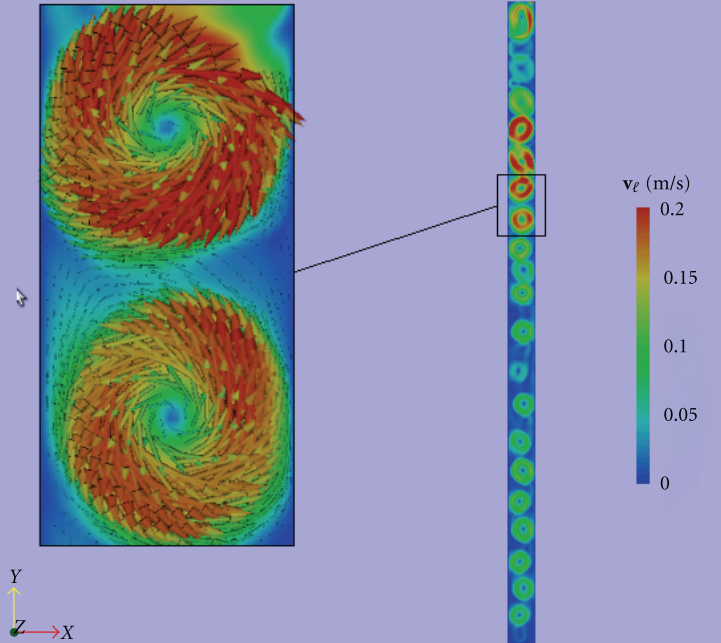
\includegraphics[width=\textwidth]{pseudoalex.png}
    \caption{The velocity magnitude contour in the quiescent channel from Alexiadis \cite{Alexiadis2012a}, the geometry is the same with the one in this work, while $i_{av} = 500 \, \mathrm{A/m^2}$}
    \label{pseudoalex}
\end{figure}

In another simulation done in COMSOL using the bubbly, the same bubbly flow model discussed in section \ref{section:bubblyflowmodel}, the similar pseudo turbulence behaviour is observed, as shown in figure \ref{pseudocirculat}. 

There is an important difference between the simulation results in figure \ref{pseudocirculat} and the work of Alexiadius: in this longer channel, this pseudo-turbulence behaviour only happens when the channel is \textbf{wide} enough, while from the correlation given by Alexiadius the pseudo-turbulence tends to be triggered when the channel width decreases. As a matter of fact, the contour in figure \ref{pseudocirculat} is an accidental finding, since the solver failed to reach the steady-state solution once this pseudo-turbulence starts to emerge, and for $i_{av} = 1000 \, A/m^2$, this happens when the channel width grows larger than $2 \, \mathrm{cm}$. The failing of steady-state simulation makes sense if the pseudo-turbulence phenomena could be confirmed since in the previous simulation done in OpenFOAM it is found that the pseudo-turbulence solution is periodic, which is intrinsically unsteady.

\begin{figure}[H]
    \centering
    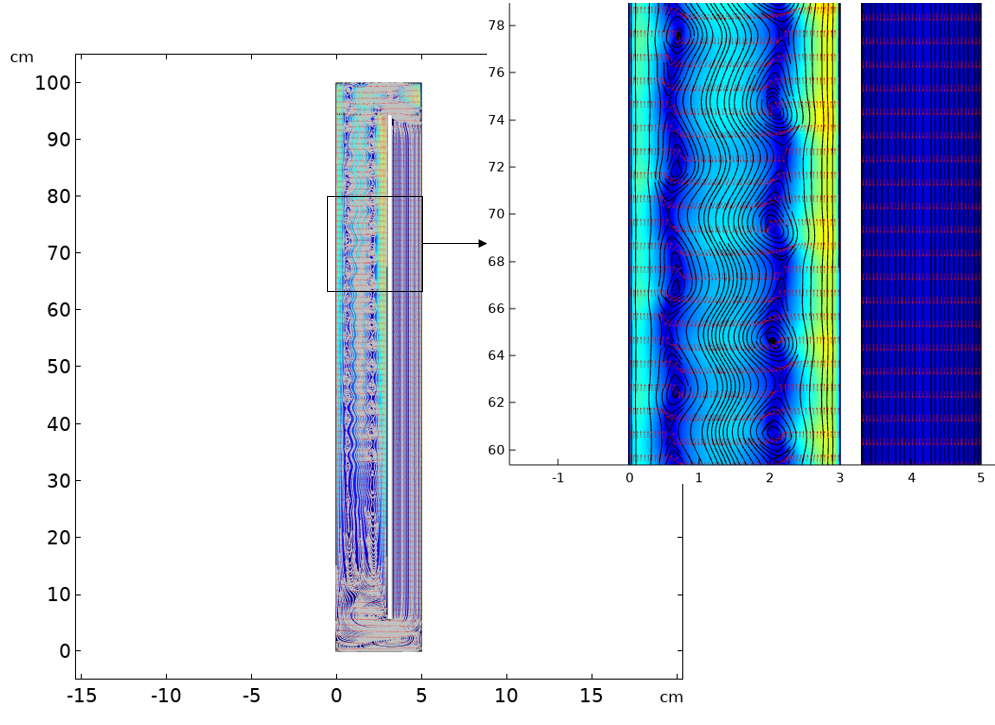
\includegraphics[width=\textwidth]{pseudocirculat.png}
    \caption{The similar pseudo-turbulence behaviour in the long circulating channel, in this model gases are evolved from both sides of the channel, with $i_{av} = 1000 \, \mathrm{A/m^2}$, $N_{gasright} = - \frac{RTi_{av}}{2pF}$, $N_{gasleft} = \frac{RTi_{av}}{4pF}$, the flow is also purely driven by the bubbles}
    \label{pseudocirculat}
\end{figure}

\section*{Extra 1d velocity and volume fraction profiles}

\begin{figure}[H]
    \centering
    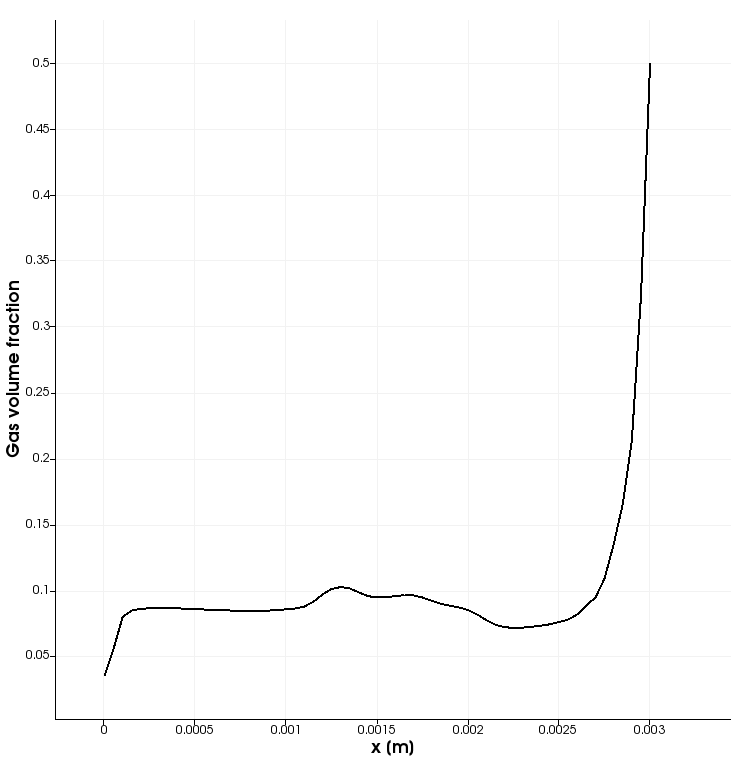
\includegraphics[width = 0.5\textwidth]{volumeprofileappendix.png}
    \caption{The volume fraction profile at $y = 30 \, \mathrm{mm}$ in the quiescent channel shown in figure \ref{appendixgeometry1}, $i_{av}=1000 \, \mathrm{A/m^2}$}
    \label{pseudovolume}
\end{figure}

\begin{figure}
\centering
\begin{subfigure}{.43\textwidth}
  \centering
  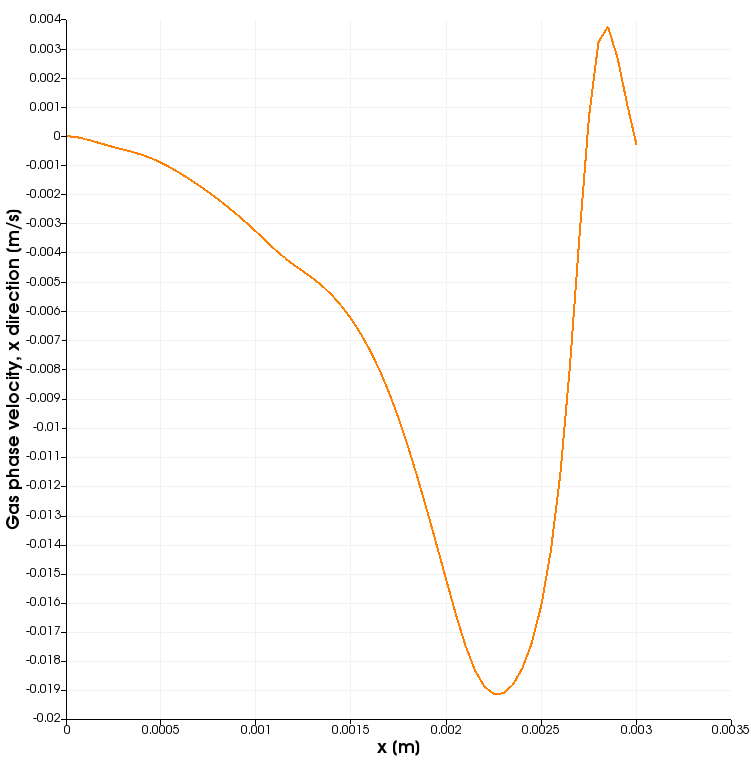
\includegraphics[width=1\linewidth]{gasphasevelocityxdirection.png}
  \caption{Gas phase velocity at x-direction}
\end{subfigure}%
\begin{subfigure}{.43\textwidth}
  \centering
  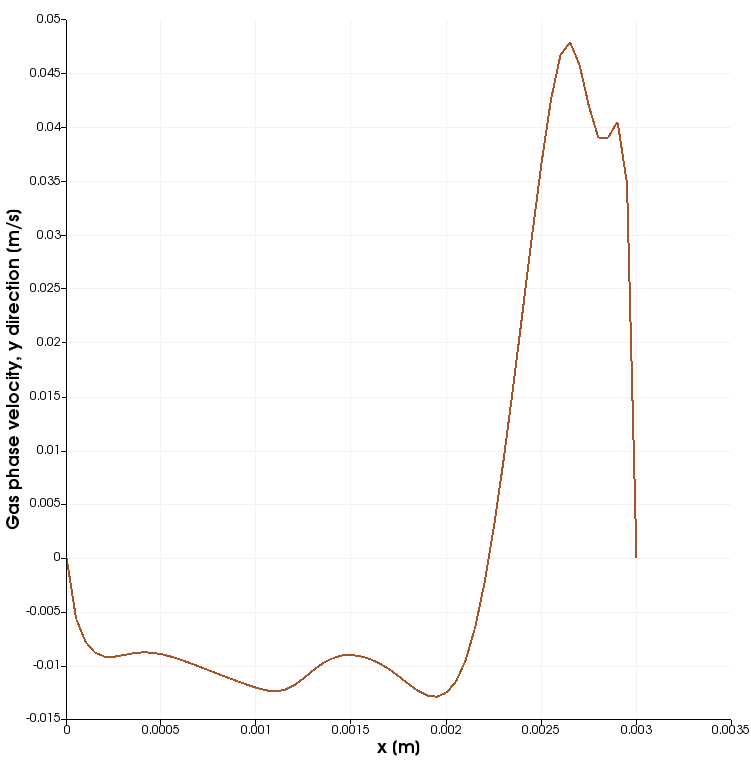
\includegraphics[width=1\linewidth]{gasphasevelocityydirection.png}
  \caption{Gas phase velocity at y-direction}
\end{subfigure}
\begin{subfigure}{.43\textwidth}
  \centering
  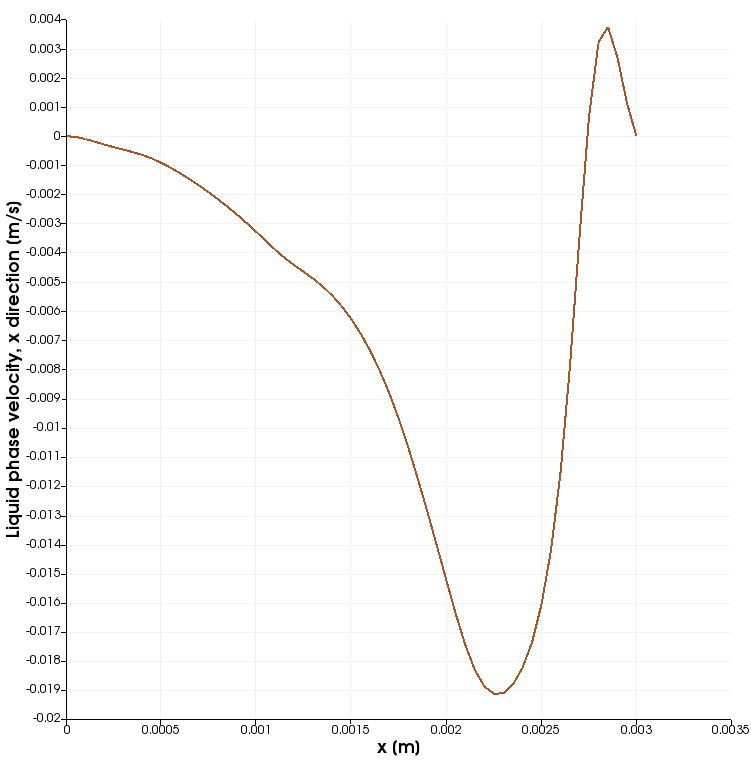
\includegraphics[width=1\linewidth]{liquidphasevelocityxdirection.png}
  \caption{Liquid phase velocity at x-direction}
\end{subfigure}%
\begin{subfigure}{.43\textwidth}
  \centering
  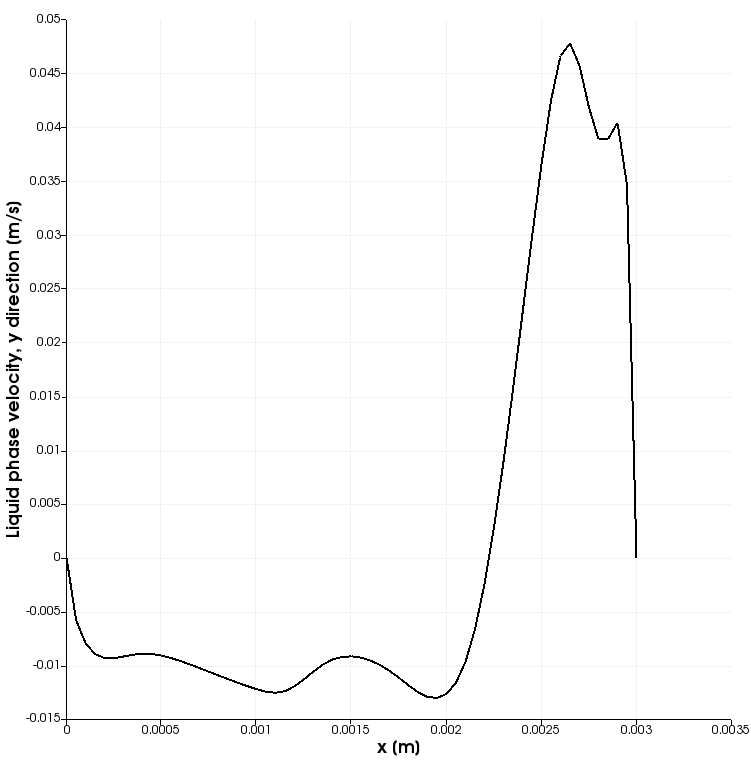
\includegraphics[width=1\linewidth]{liquidphasevelocityydirection.png}
  \caption{Liquid phase velocity at y-direction}
\end{subfigure}
\caption{The velocity profile at $y = 30 \, \mathrm{mm}$ in the quiescent channel shown in figure \ref{appendixgeometry1}, $i_{av}=1000 \, \mathrm{A/m^2}$}
\label{pseudovelocity}
\end{figure}